\section{Result Analysis}
\label{sec:ResultAnalysis}

%comparar as duas cenas
%introduzir o octave optimizado, seguindo a linha de raciocinio do ngspice
%comparar as tabelinhas de output dos dois lados, expicar porque diferem.

\indent

In this section the results will firstly be analysed and then compared, identifying the differences between the calculated results and the simulation results. 

The {\it Octave} graph with optimised parameters will be presented and discussed in this section. This final graph (Figure \ref{fig:OutputOC}) can be obtained by introducing these optimised parameters on the previous {\it script}.

\paragraph*{Note:}
When running the simulation it is possible to notice that it takes a while to plot the graphics. This is due to the fact that the number of time instants used is very high. If it were lower, the graph of the exponentially decaying voltage (from the capacitor) would not intercept the module of the sinusoidal voltage's (output of the bridge rectifier) graph. In turn, that would increase the error by making an approximation in order to force this interception, which looked like a vertical line when analysing the ripple's graph up close.

\subsection{Graphs}
\subsubsection{Outputs overview}

\begin{figure}[H]
\centering
\begin{subfigure}{.5\textwidth}
  \centering
  \includegraphics[width=.95\linewidth]{ACDC_converter_Optimized.eps}
  \caption{Octave}
  \label{fig:OutputOC}
\end{subfigure}%
\begin{subfigure}{.5\textwidth}
  \centering
  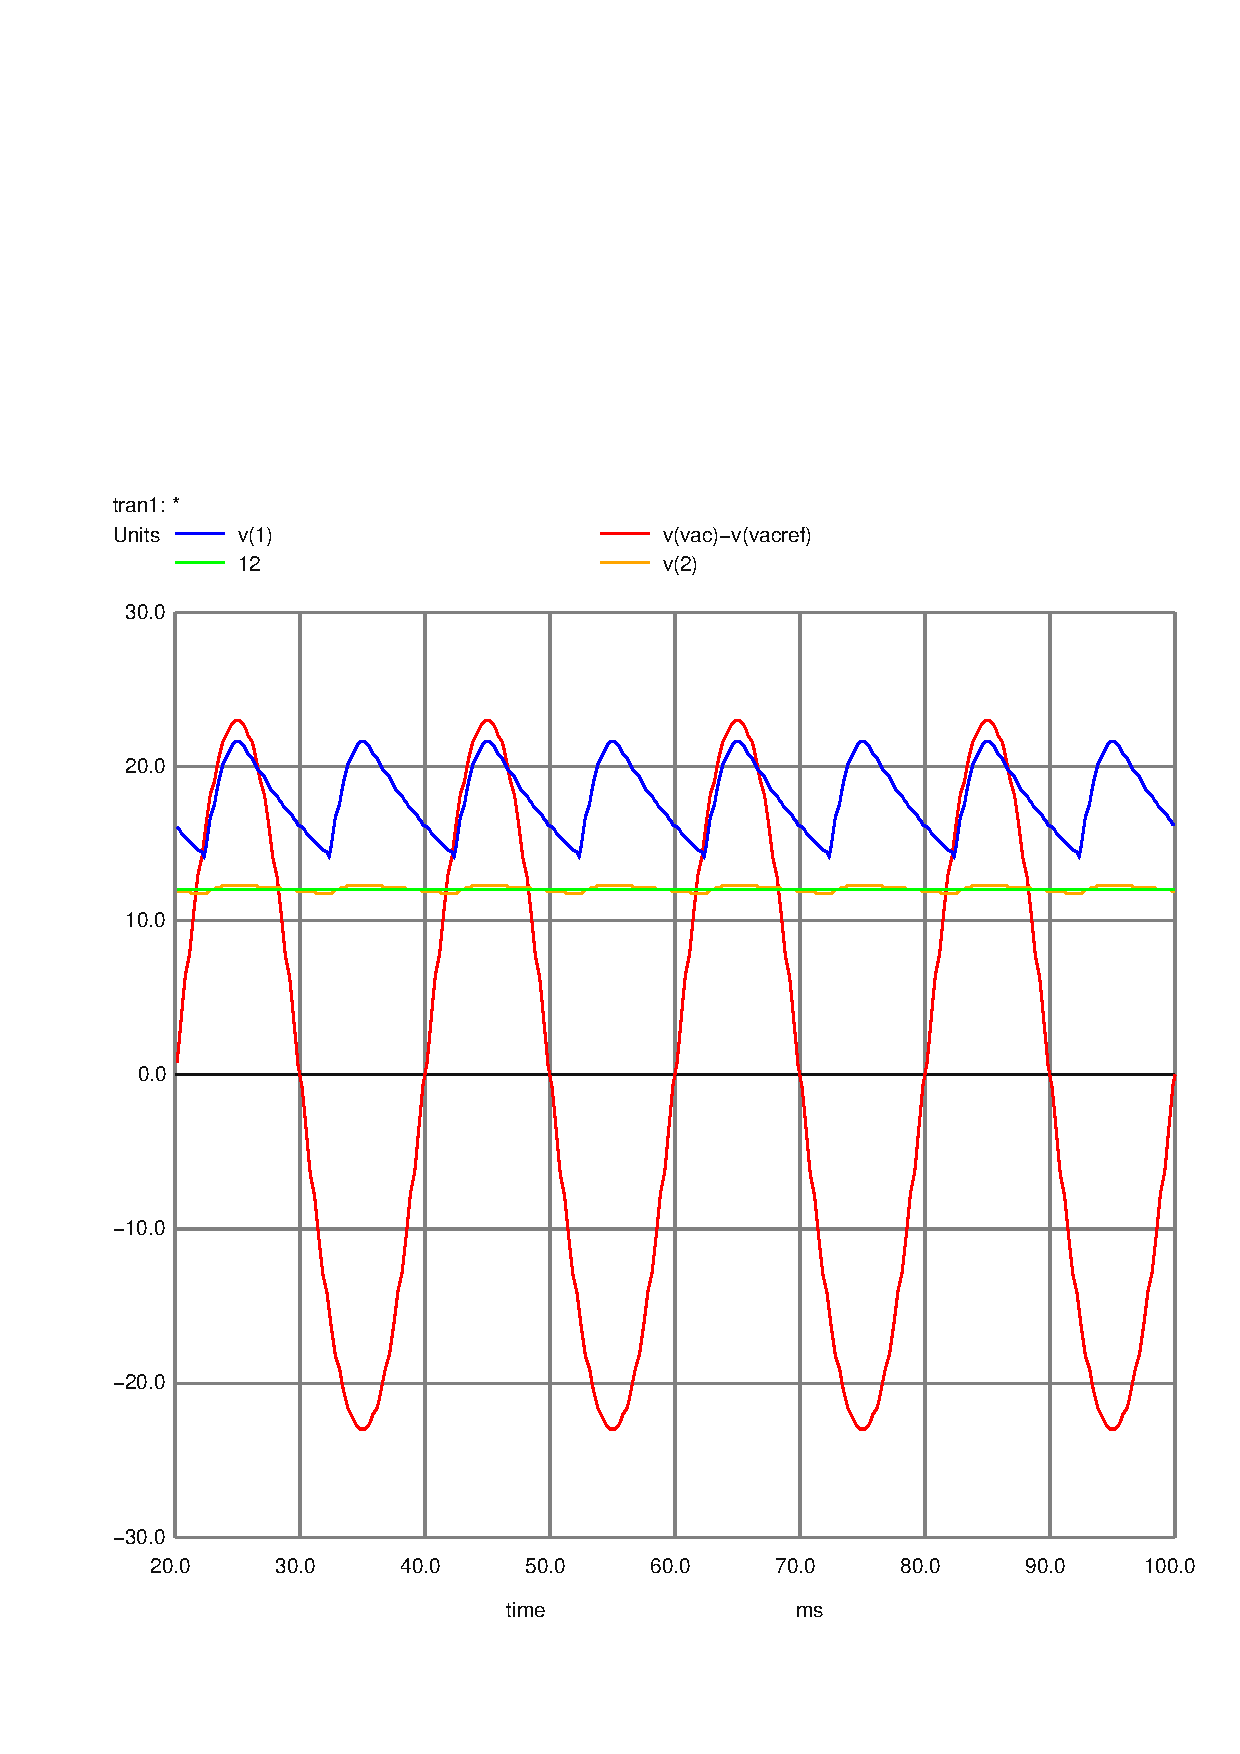
\includegraphics[width=.75\linewidth, trim={2cm 1.5cm 0.5cm 6cm}, clip]{../Simulation/sim1.pdf}
  \caption{Ngspice}
  \label{fig:OutputNG}
\end{subfigure}
\caption{General voltage output}
\label{fig:Output}
\end{figure}

\indent

In these graphs we can see that the results match almost identically, as expected. However there is a very slight deviation from 12 V on the Figure \ref{fig:OutputOC}. This does not happen on the one Generated using \textit{NGSpice}, it matches 12 volts almost perfectly.

\subsubsection{Outputs closeup overview}

\begin{figure}[H]
\centering
\begin{subfigure}{.5\textwidth}
  \centering
  \includegraphics[width=.95\linewidth]{Ripple_Optimized.eps}
  \caption{Octave}
\end{subfigure}%
\begin{subfigure}{.5\textwidth}
  \centering
  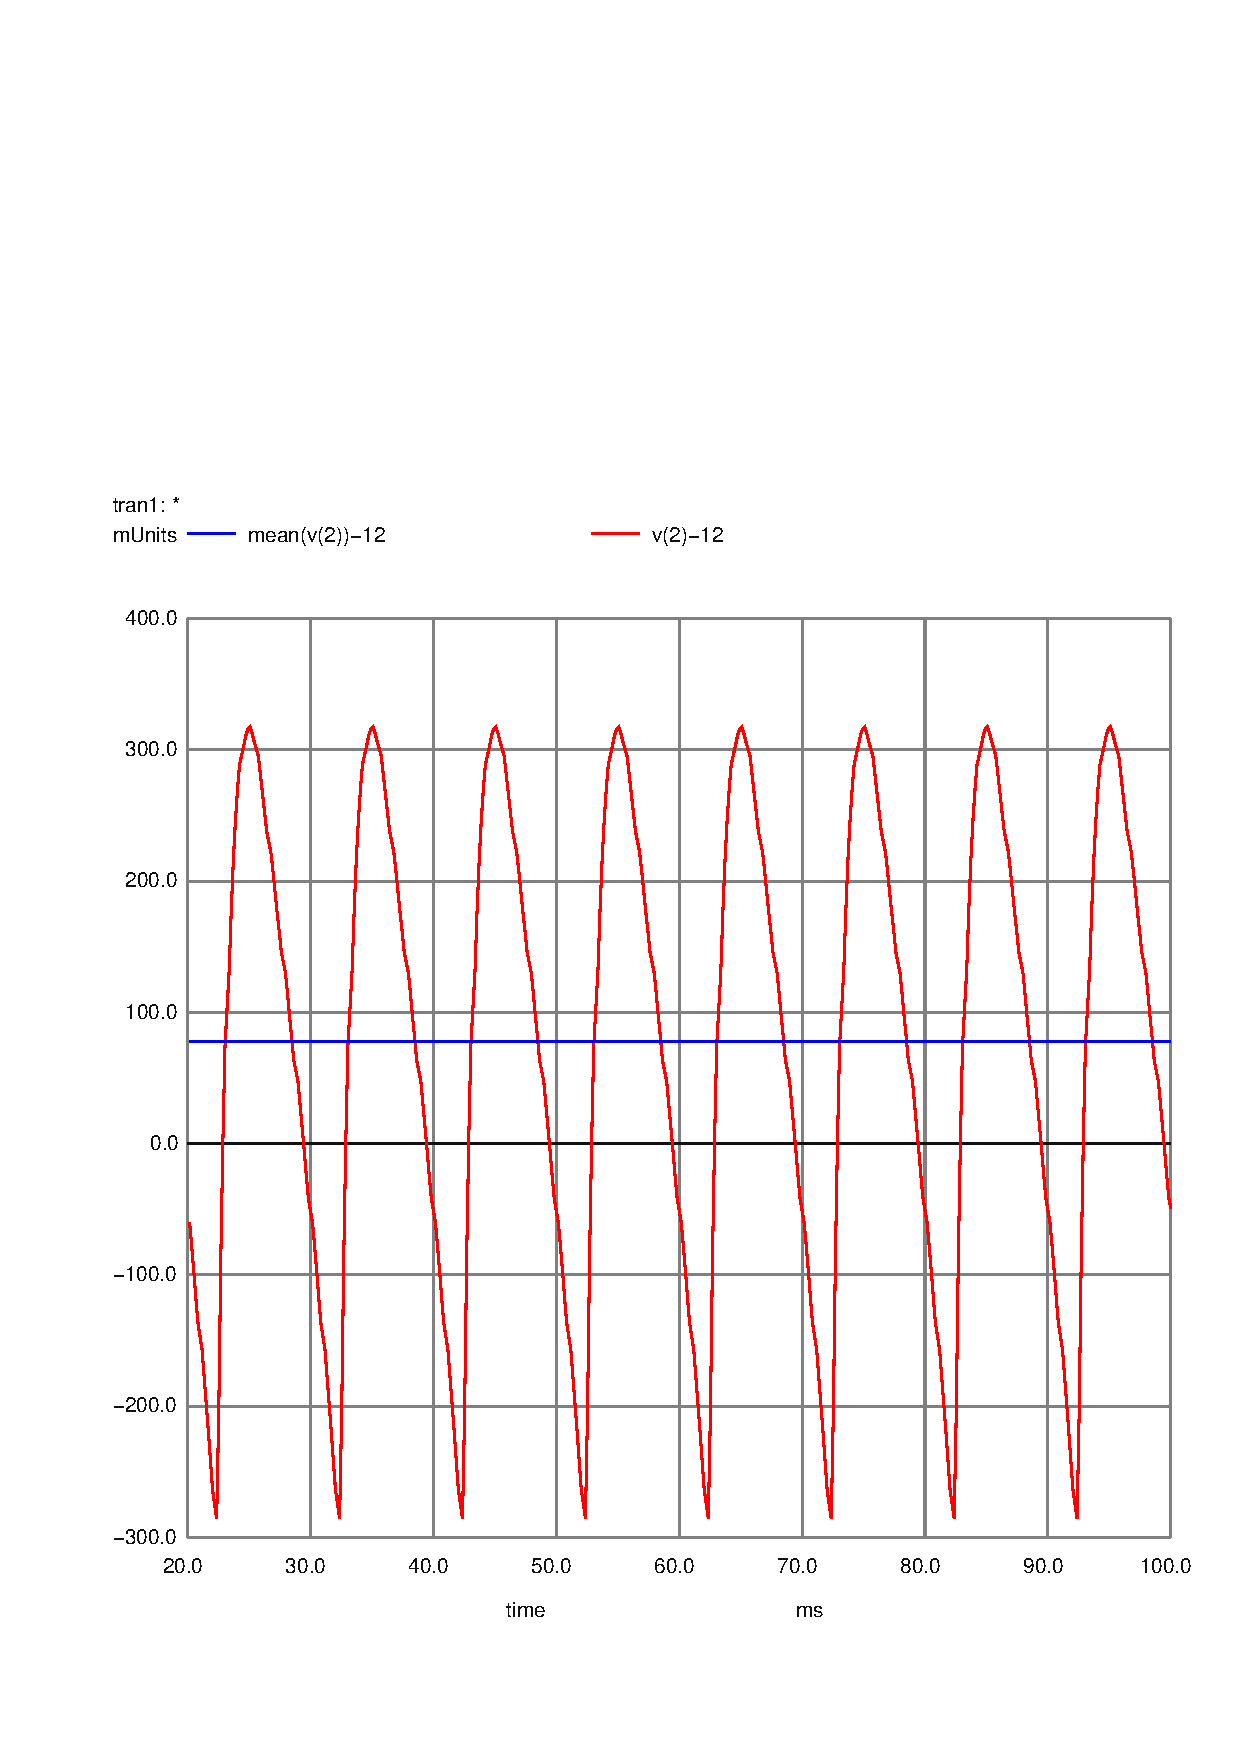
\includegraphics[width=.75\linewidth, trim={2cm 1.5cm 0.5cm 6cm}, clip]{../Simulation/sim2.pdf}
  \caption{Ngspice}
\end{subfigure}
\caption{Voltage ripple and average close up}
\label{fig:OutputCloseUp}
\end{figure}

\indent

Similarly to what happened on the previous graph, we can clearly see that the mean voltage deviation on the \textit{Octave} graph differs a lot from the pretended $0V$ (This means the average voltage is not close to $12V$), this does not happen on the \textit{Ngspice} version, it matches perfectly.
On the voltage ripple, the differences are not that severe, but it is present. 

These are expected since on \textit{Octave}, approximations were used, which deteriorate the results.


\subsection{Tables}



\begin{table}[H]
    \caption{Output parameters}
    \begin{subtable}{.5\linewidth}
      \centering
        \caption{Octave}
        \begin{tabular}{ll}
        \hline    
        {\bf Name} & {\bf Value} \\ \hline
        \input{../Analysis/OutputResults_Op.tex}
        \end{tabular}
        \label{tab:OutParamOc}
    \end{subtable}%
    \begin{subtable}{.5\linewidth}
      \centering
        \caption{Ngspice}
        \begin{tabular}{ll}
        \hline    
        {\bf Name} & {\bf Value} \\ \hline
        @gcs[i] & 1.837491e-04\\ \hline
@id[current] & 1.033653e-03\\ \hline
@r1[i] & 1.924024e-04\\ \hline
@r2[i] & 1.837491e-04\\ \hline
@r3[i] & 8.653299e-06\\ \hline
@r4[i] & -1.14368e-03\\ \hline
@r5[i] & 8.499042e-04\\ \hline
@r6[i] & 9.512771e-04\\ \hline
@r7[i] & 9.512771e-04\\ \hline
v(1) & 5.008942e+00\\ \hline
v(2) & 4.811140e+00\\ \hline
v(3) & 4.437766e+00\\ \hline
v(4) & 0.000000e+00\\ \hline
v(5) & 4.785125e+00\\ \hline
v(6) & 2.133477e+00\\ \hline
v(7) & -1.98683e+00\\ \hline
v(8) & -2.93853e+00\\ \hline
}
        \end{tabular}
        \label{tab:OutParamNG}
    \end{subtable} 
    \label{tab:OutParam}
\end{table}






\indent

Looking at these tables it is possible to confirm what was said before. While the ripple only differs in one order of magnitude from the simulation values to the theoretical ones, the mean voltage deviation differs in five orders of magnitude (where the simulation values are the smallest).

As previously stated, the differences came from approximations such as the diode model approximation, since the diode equation (equation \ref{eq:DiodeEq}) was not solved. Instead, $V_{on}$ was used to calculate the voltage output at the envelope detector. The most probable source of error was overestimating $V_{on}$, since the values at the output, on this section, are bellow of what was expected from \textit{Ngspice}. This happens because $V_o= V_s-2V_{on}$, where $V_o$ is the output voltage and $V_s$ is the input one. 

Another source of error may come from the computation of the voltage exponential decay, from the capacitor after the bridge rectifier. It was calculated using equation \ref{eq:toff} and \ref{eq:vc}, which means that $t_{off}$ depends on $V_{on}$ and therefore might be different from the real one. $v_O(t)$ may differ too, due to the dependencies on $t_{off}$ and $V_{on}$.
